\section{Componiendo nudos.}\label{seccion3}
Supongamos que tenemos dos proyecciones J y K de nudos. Podemos definir un nuevo nudo a partir de ellos eliminando un arco de cada una de las proyecciones y conectando los 4 extremos finales de dos en dos mediante otros arcos de modo que no se añadan ni eliminen cruces.\\
A este nudo resultante le llamaremos \textbf{suma conexa} o composición de los dos nudos y se denotará como \textbf{J\#K}. A los nudos originales J y K les llamaremos \textbf{nudos factores}. \\

Por ejemplo, consideremos como nudos factores el nudo trébol y el nudo de ocho. 
\begin{figure}[h!]
	\subfigure[J]{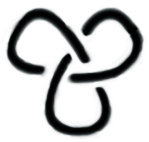
\includegraphics[width=2.5cm]{inudos/conexion1.jpg}} 
	\subfigure[K]{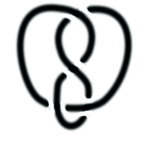
\includegraphics[width=2.5cm]{inudos/fig8.jpg}}
	\centering
	\caption{Nudo trébol y nudo de ocho.}
	\label{comp1} 
\end{figure}

Haciendo la suma conexa de ambos nudos obtenemos el nudo composición:
\begin{figure}[h!]
	\subfigure[Haciendo la composición]{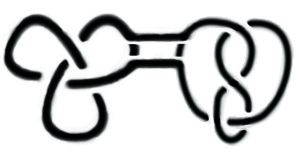
\includegraphics[width=7cm]{inudos/conexion2.jpg} }
	\subfigure[J\#K]{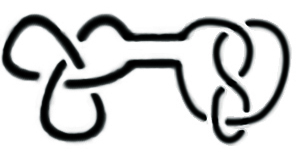
\includegraphics[width=7cm]{inudos/conexion3.jpg}}
	\centering
	\caption{Composición de nudo trébol y nudo de ocho.}
	\label{comp2} 
\end{figure}


El nudo trivial es un elemento identidad para la suma conexa: si hacemos la composición de un nudo cualquiera J con el nudo trivial, vamos a obtener el propio nudo J. Por ejemplo, seguimos considerando J como el nudo trébol y el nudo trivial como K. \\
\begin{figure}[h!]
	\centering
	\subfigure[J]{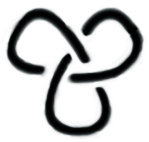
\includegraphics[width=2.5cm]{inudos/conexion1.jpg} }
	\subfigure[K]{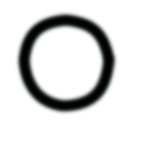
\includegraphics[width=2.5cm]{inudos/1.jpg}}
	\caption{Nudo trébol y nudo trivial.}
	\label{comp3} 
\end{figure}

Su suma conexa nos seguiría dando el nudo factor J, es decir, el nudo trébol.\\

\begin{figure}[h!]
	\subfigure[Haciendo la composición]{
\includegraphics[width=8cm]{inudos/conexion4.jpg} }
	\subfigure[J\#K]{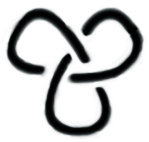
\includegraphics[width=4cm]{inudos/conexion1.jpg}}
	\centering
	\caption{Composición de nudo trébol y nudo trivial.}
	\label{comp4} 
\end{figure}

\underline{\textbf{ Definición:}}\\
Diremos que un \textbf{nudo es primo} si no puede ser expresado como la suma conexa de dos nudos, a menos que uno de ellos sea el nudo trivial. \\

\underline{ \textbf{ Definición:}}\\
Diremos que un \textbf{nudo es compuesto} si no es el nudo trivial ni es un nudo primo.\\

Por ejemplo, los nudos trébol y nudo de ocho de la figura \ref{comp1} son nudos primos mientras que el nudo de la figura \ref{comp2} es un nudo compuesto. \\ 

Hay una gran variedad de nudos primos. Cualquier nudo puede ser expresado singularmente como suma conexa de nudos primos. En la tabla \ref{comp6}, extraida de \cite{10}, podemos ver los diferentes nudos primos que tienen menos de 8 cruces.\\
\begin{figure}[h!]
	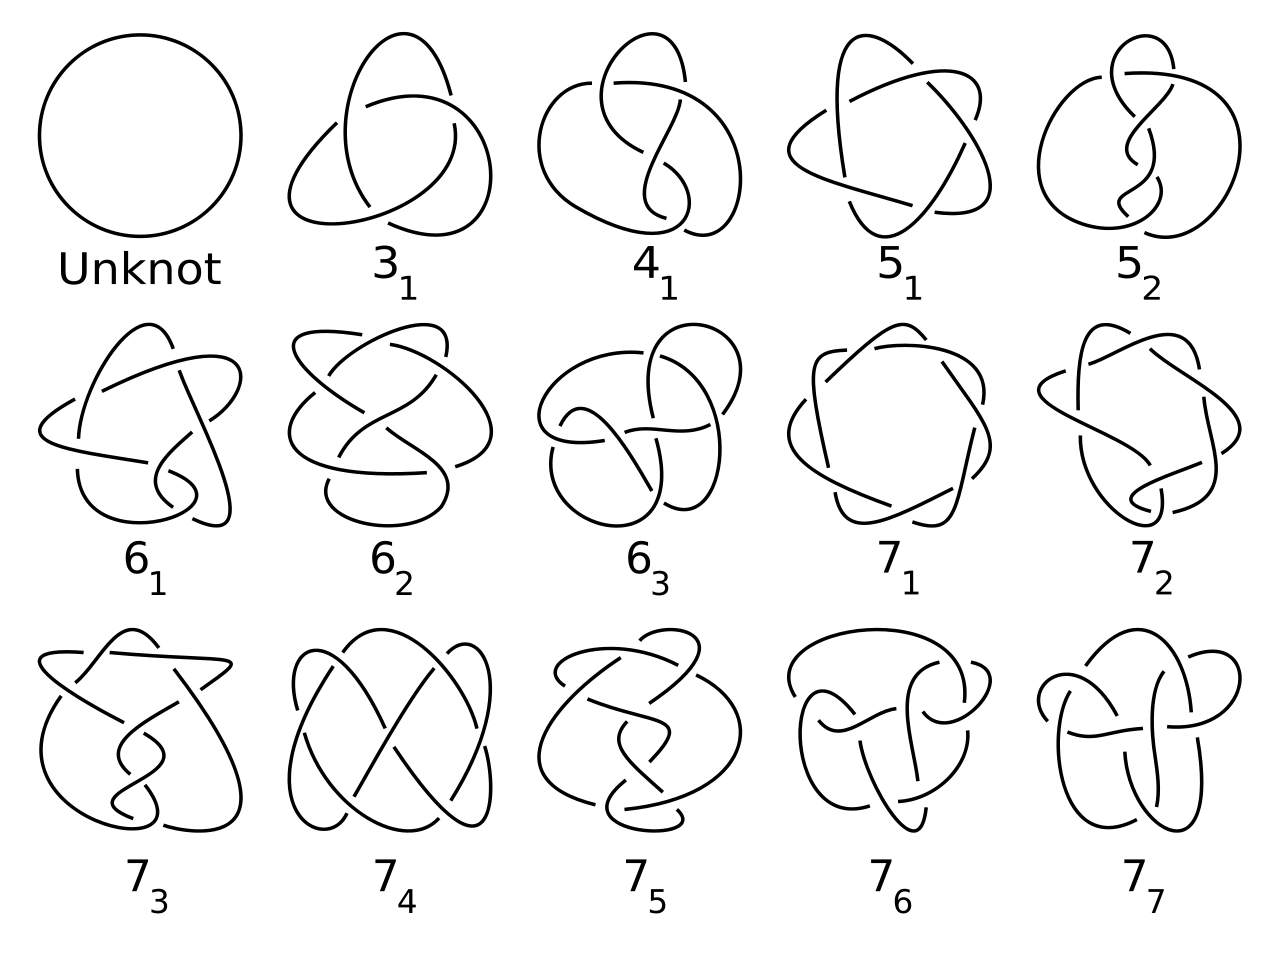
\includegraphics[width=14cm]{inudos/tableknot.png}
	\centering
	\caption{Tabla de nudos primos.}
	\label{comp6} 
\end{figure}




Finalmente, es importante destacar el hecho de que la elección que hacemos de los arcos que eliminamos de cada uno de los nudos factores afecta al nudo composición. Por tanto, es posible construir dos nudos composición diferentes a partir del mismo par de nudos factores. Veamos esta idea con más detalle, para ello necesitamos:\\

\underline{\textbf{ Definición:}}\\
\textbf{ Un nudo orientado} es un nudo al que se le ha asignado una orientación, es decir, es un nudo que dispone de una dirección de viaje sobre él mismo. Esta orientación se indica mediante flechas en la proyección. \\

\underline{\textbf{ Definición:}}\\
\textbf{ Un nudo es invertible} si es equivalente a sí mismo con la orientación opuesta. \\

El problema de determinar si un nudo cualquiera es o no invertible no es para nada trivial.

Como ejemplo de nudo invertible nos podemos encontrar el nudo trébol, que vemos en la imagen \ref{comp5}.\\
\begin{figure}[h!]
	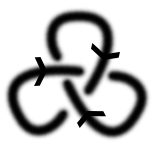
\includegraphics[width=3.5cm]{inudos/3fcon1.png}
	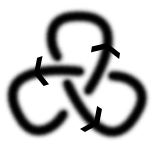
\includegraphics[width=3.5cm]{inudos/3fcon2.png}
	\centering
	\caption{Ambas orientaciones del nudo trébol.}
	\label{comp5} 
\end{figure}

Sean los dos nudos factores J y K a los que se asignamos una orientación. Tendremos dos formas posibles de hacer la composición: conectar con las orientaciones emparejadas o no emparejadas. \\
Todas las composiciones de los nudos cuyas orientaciones emparejan al componer, darán el mismo nudo composición. Todas las composiciones de los nudos cuyas orientaciones no emparejan al componer, también darán el mismo nudo composición. Sin embargo, es posible que la composición de los nudos cuyas orientaciones emparejen no de lugar al mismo nudo que haciendo la composición de los nudos cuyas orientaciones no emparejen. Serán el mismo si uno de los nudos factores es invertible.\\

Veamos un caso en el que la composición de dos mismos factores, genera nudos diferentes. Consideramos el nudo de la imagen \ref{comp7}.\\

\begin{figure}[h!]
	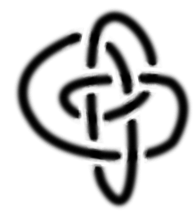
\includegraphics[width=4cm]{inudos/817con.png}
	\centering
	\caption{Nudo factor J y K.}
	\label{comp7} 
\end{figure}
Si componemos el nudo consigo mismo conectando las orientaciones emparejadas y desemparejadas obtenemos nudos que no son equivalentes. Lo podemos comprobar visualmente en la Figura \ref{comp8}.

\begin{figure}[h!]
	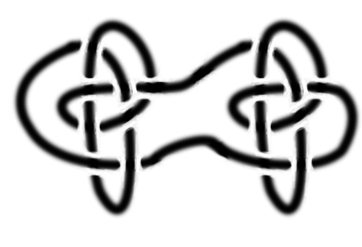
\includegraphics[width=7cm]{inudos/817def1.png}
	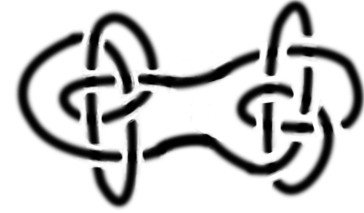
\includegraphics[width=7cm]{inudos/817def2.png}
	\centering
	\caption{Las composiciones no son equivalentes.}
	\label{comp8} 
\end{figure}